\documentclass[11pt,preprint]{elsarticle}

\usepackage{lmodern}
%%%% My spacing
\usepackage{setspace}
\setstretch{1.2}
\DeclareMathSizes{12}{14}{10}{10}

% Wrap around which gives all figures included the [H] command, or places it "here". This can be tedious to code in Rmarkdown.
\usepackage{float}
\let\origfigure\figure
\let\endorigfigure\endfigure
\renewenvironment{figure}[1][2] {
    \expandafter\origfigure\expandafter[H]
} {
    \endorigfigure
}

\let\origtable\table
\let\endorigtable\endtable
\renewenvironment{table}[1][2] {
    \expandafter\origtable\expandafter[H]
} {
    \endorigtable
}


\usepackage{ifxetex,ifluatex}
\usepackage{fixltx2e} % provides \textsubscript
\ifnum 0\ifxetex 1\fi\ifluatex 1\fi=0 % if pdftex
  \usepackage[T1]{fontenc}
  \usepackage[utf8]{inputenc}
\else % if luatex or xelatex
  \ifxetex
    \usepackage{mathspec}
    \usepackage{xltxtra,xunicode}
  \else
    \usepackage{fontspec}
  \fi
  \defaultfontfeatures{Mapping=tex-text,Scale=MatchLowercase}
  \newcommand{\euro}{€}
\fi

\usepackage{amssymb, amsmath, amsthm, amsfonts}

\def\bibsection{\section*{References}} %%% Make "References" appear before bibliography


\usepackage[numbers]{natbib}

\usepackage{longtable}
\usepackage[margin=2.3cm,bottom=2cm,top=2.5cm, includefoot]{geometry}
\usepackage{fancyhdr}
\usepackage[bottom, hang, flushmargin]{footmisc}
\usepackage{graphicx}
\numberwithin{equation}{section}
\numberwithin{figure}{section}
\numberwithin{table}{section}
\setlength{\parindent}{0cm}
\setlength{\parskip}{1.3ex plus 0.5ex minus 0.3ex}
\usepackage{textcomp}
\renewcommand{\headrulewidth}{0.2pt}
\renewcommand{\footrulewidth}{0.3pt}

\usepackage{array}
\newcolumntype{x}[1]{>{\centering\arraybackslash\hspace{0pt}}p{#1}}

%%%%  Remove the "preprint submitted to" part. Don't worry about this either, it just looks better without it:
\makeatletter
\def\ps@pprintTitle{%
  \let\@oddhead\@empty
  \let\@evenhead\@empty
  \let\@oddfoot\@empty
  \let\@evenfoot\@oddfoot
}
\makeatother

 \def\tightlist{} % This allows for subbullets!

\usepackage{hyperref}
\hypersetup{breaklinks=true,
            bookmarks=true,
            colorlinks=true,
            citecolor=blue,
            urlcolor=blue,
            linkcolor=blue,
            pdfborder={0 0 0}}


% The following packages allow huxtable to work:
\usepackage{siunitx}
\usepackage{multirow}
\usepackage{hhline}
\usepackage{calc}
\usepackage{tabularx}
\usepackage{booktabs}
\usepackage{caption}


\newenvironment{columns}[1][]{}{}

\newenvironment{column}[1]{\begin{minipage}{#1}\ignorespaces}{%
\end{minipage}
\ifhmode\unskip\fi
\aftergroup\useignorespacesandallpars}

\def\useignorespacesandallpars#1\ignorespaces\fi{%
#1\fi\ignorespacesandallpars}

\makeatletter
\def\ignorespacesandallpars{%
  \@ifnextchar\par
    {\expandafter\ignorespacesandallpars\@gobble}%
    {}%
}
\makeatother


% definitions for citeproc citations
\NewDocumentCommand\citeproctext{}{}
\NewDocumentCommand\citeproc{mm}{%
\href{\#cite.\detokenize{#1}}{#2}\nocite{#1}}

\makeatletter
% allow citations to break across lines
\let\@cite@ofmt\@firstofone
% avoid brackets around text for \cite:
\def\@biblabel#1{}
\def\@cite#1#2{{#1\if@tempswa , #2\fi}}
\makeatother
\newlength{\cslhangindent}
\setlength{\cslhangindent}{1.5em}
\newlength{\csllabelwidth}
\setlength{\csllabelwidth}{3em}
\newenvironment{CSLReferences}[2] % #1 hanging-indent, #2 entry-spacing
{\begin{list}{}{%
	\setlength{\itemindent}{0pt}
	\setlength{\leftmargin}{0pt}
	\setlength{\parsep}{0pt}
	% turn on hanging indent if param 1 is 1
	\ifodd #1
	\setlength{\leftmargin}{\cslhangindent}
	\setlength{\itemindent}{-1\cslhangindent}
	\fi
	% set entry spacing
	\setlength{\itemsep}{#2\baselineskip}}}
{\end{list}}

\usepackage{calc}
\newcommand{\CSLBlock}[1]{\hfill\break\parbox[t]{\linewidth}{\strut\ignorespaces#1\strut}}
\newcommand{\CSLLeftMargin}[1]{\parbox[t]{\csllabelwidth}{\strut#1\strut}}
\newcommand{\CSLRightInline}[1]{\parbox[t]{\linewidth - \csllabelwidth}{\strut#1\strut}}
\newcommand{\CSLIndent}[1]{\hspace{\cslhangindent}#1}


\urlstyle{same}  % don't use monospace font for urls
\setlength{\parindent}{0pt}
\setlength{\parskip}{6pt plus 2pt minus 1pt}
\setlength{\emergencystretch}{3em}  % prevent overfull lines
\setcounter{secnumdepth}{5}

%%% Use protect on footnotes to avoid problems with footnotes in titles
\let\rmarkdownfootnote\footnote%
\def\footnote{\protect\rmarkdownfootnote}
\IfFileExists{upquote.sty}{\usepackage{upquote}}{}

%%% Include extra packages specified by user
\usepackage{sectsty}
\sectionfont{\bfseries\large}
\subsectionfont{\bfseries\normalsize}

%%% Hard setting column skips for reports - this ensures greater consistency and control over the length settings in the document.
%% page layout
%% paragraphs
\setlength{\baselineskip}{12pt plus 0pt minus 0pt}
\setlength{\parskip}{12pt plus 0pt minus 0pt}
\setlength{\parindent}{0pt plus 0pt minus 0pt}
%% floats
\setlength{\floatsep}{12pt plus 0 pt minus 0pt}
\setlength{\textfloatsep}{20pt plus 0pt minus 0pt}
\setlength{\intextsep}{14pt plus 0pt minus 0pt}
\setlength{\dbltextfloatsep}{20pt plus 0pt minus 0pt}
\setlength{\dblfloatsep}{14pt plus 0pt minus 0pt}
%% maths
\setlength{\abovedisplayskip}{12pt plus 0pt minus 0pt}
\setlength{\belowdisplayskip}{12pt plus 0pt minus 0pt}
%% lists
\setlength{\topsep}{10pt plus 0pt minus 0pt}
\setlength{\partopsep}{3pt plus 0pt minus 0pt}
\setlength{\itemsep}{5pt plus 0pt minus 0pt}
\setlength{\labelsep}{8mm plus 0mm minus 0mm}
\setlength{\parsep}{\the\parskip}
\setlength{\listparindent}{\the\parindent}
%% verbatim
\setlength{\fboxsep}{5pt plus 0pt minus 0pt}



\begin{document}



\begin{frontmatter}  %

\title{Macroeconomics Assignment}

% Set to FALSE if wanting to remove title (for submission)




\author[Add1]{Liam Andrew Beattie}
\ead{22562435@sun.ac.za}





\address[Add1]{Macroeconomics 871, Stellenbosch University, South
Africa}


\begin{abstract}
\small{
Almost an abstract
}
\end{abstract}

\vspace{1cm}





\vspace{0.5cm}

\end{frontmatter}

\setcounter{footnote}{0}



%________________________
% Header and Footers
%%%%%%%%%%%%%%%%%%%%%%%%%%%%%%%%%
\pagestyle{fancy}
\chead{}
\rhead{}
\lfoot{}
\rfoot{\footnotesize Page \thepage}
\lhead{}
%\rfoot{\footnotesize Page \thepage } % "e.g. Page 2"
\cfoot{}

%\setlength\headheight{30pt}
%%%%%%%%%%%%%%%%%%%%%%%%%%%%%%%%%
%________________________

\headsep 35pt % So that header does not go over title




I have used an R package from Mati (\citeproc{ref-Mati2019}{2019}) and
should give credit. This allowed me to code everything in R while still
using Dynare.

\[r^B_{t-1} = R^B_{t-1}/\pi_t\]

\section{Model Specification}\label{model-specification}

\begin{equation}
\pi_t = \frac{P_t}{P_{t-1}}
\label{inflation}
\end{equation}

\begin{equation}
c_t = \frac{C_t}{P_t}, 
\quad i_t = \frac{I_t}{P_t}, 
\quad g_t = \frac{G_t}{P_t},
\quad b_t = \frac{B_t}{P_t}
\label{real_conversions}
\end{equation}

Above could note be a heading on itself. Just a paragraph that it is a
core rbc foundations and what that means.

As with \eqref{real_conversions}, it is a general rule that capital
letters denote nominal amounts and lowercase denote real values, however
to follow convention \(K_t\) denotes real capital.

Mainly adding capital to Sims
(\citeproc{ref-sims2024newkeynesian}{2024a}), while also introducing
adjustment costs from Sims (\citeproc{ref-sims2024rbc}{2024b}) .
Rotemberg prices was used while gleeming insights from European Central
Bank (\citeproc{ref-ecbwp770}{2022}) .

\subsection{Households}\label{households}

\(c_t,\,h_t,\,m_t,\,b_t,\,K_t,\,i_t\) are all real values for
consumption, hours worked, money, bonds, capital, and investment.

\begin{equation}
\max_{\{c_t,\,h_t,\,m_t,\,b_t,\,K_t,\,i_t\}}
\mathbb{E}_0 \sum_{t=1}^{\infty} \beta^{t-1}
\left[
\frac{\Bigl(c_t - \eta\,c_{t-1}\Bigr)^{1-\theta}}{1-\theta}
\;-\;\chi\,\frac{h_t^{1+\gamma}}{1+\gamma}
\;+\;\psi\,\ln\!\Bigl(m_t\Bigr)
\right]
\label{lifetime_utility_real}
\end{equation}

\begin{equation}
c_t + i_t + b_t + m_t \leq r^B_{t-1}b_{t-1} + \dfrac{m_{t-1}}{\pi_t} + w_t h_t + r^k_t K_{t-1} + \Pi^r_t - \tau_t
\label{flow_constraint_real}
\end{equation}

\begin{equation}
K_t
\;=\;
(1 - \delta)\,K_{t-1}
\;+\; i_t
\;-\;\frac{\phi_k}{2}
\left(\frac{i_t}{K_{t-1}} - \delta\right)^{2}
\,K_{t-1}
\label{capital_accumulation_real}
\end{equation}

Households are the owners of all intermediate‐goods firms and receive
the aggregate profits as lump‐sum income transfers each period. Denoting
aggregate real profits by \(\Pi^r_t\), we can write

\begin{equation}
\Pi^r_t = Y_t - r^k_t K_{t-1} - w_t h_t - \dfrac{\phi_p}{2} (\pi_t - 1)^2 Y_t
\label{intermediate_firm_profit_real}
\end{equation}

where \(P_tY_t\) is nominal revenue, \(R^k_t K_{t-1}\) and \(W_t h_t\)
are total nominal factor payments, and the last term captures
Rotemberg‐style price adjustment costs in nominal terms.

Households maximize expected lifetime utility over consumption and
labour supply, taking all after-tax income---wages, rental income, bond
returns, and profits---as given. In particular, we treat firm profits
\(\Pi_t\) as a lump‐sum transfer from firms that enters the budget
constraint passively; households do not choose or time their utility
over firm profits, nor do they form expectations about future payouts.

From which we can derive the following first order conditions, found in
full form in Appendix \ref{household_FOC}:

\begin{equation}\label{foc_C}
\lambda_t = (c_t-\eta c_{t-1})^{-\theta} - \beta\,\eta\,\mathbb{E}_t\bigl[(c_{t+1}-\eta c_t)^{-\theta}\bigr]
\end{equation}

\begin{equation}\label{foc_h}
\lambda_t w_t = \chi h_t^{\gamma}
\end{equation}

\begin{equation}\label{foc_B}
\lambda_t = \beta \, \mathbb{E}_t \left[ \lambda_{t+1} r^B_t \right]
\end{equation}

\begin{equation}\label{foc_M}
\dfrac{\psi}{m_t} = \lambda_t - \beta \, \mathbb{E}_t \left[ \dfrac{\lambda_{t+1}}{\pi_{t+1}} \right]
\end{equation}

\begin{equation}\label{foc_I}
\lambda_t = \mu_t \left( 1 - \phi_k \left( \frac{i_t}{K_{t-1}} - \delta \right) \right)
\end{equation}

\begin{equation}\label{foc_K}
\mu_t = \beta \, \mathbb{E}_t \left[ \lambda_{t+1} r^k_{t+1} + \mu_{t+1} \left( (1-\delta) - \frac{\phi_k}{2} \left( \delta^2 - \left( \frac{i_{t+1}}{K_t} \right)^2 \right) \right) \right]
\end{equation}

\newpage

\subsection{Production}\label{production}

This model departs from standard RBC frameworks by introducing
monopolistic competition and nominal rigidities. This is achieved
through two layers of firms. The first being a perfectly competitive
final goods producers, who aggregate intermediate goods, and the second
being a monopolistically competitive intermediate goods producers with
price-setting power. This two-tiered structure captures core New
Keynesian dynamics, such as price stickiness and strategic pricing,
while retaining analytical tractability.

\subsubsection{Final Goods Producer}\label{final-goods-producer}

The final goods firm combines differentiated inputs \(Y_t(j)\) into
final output \(Y_t\) using a CES aggregator:

\begin{equation}  
Y_t = \left( \int_0^1 Y_t(j)^{\frac{\epsilon-1}{\epsilon}}  dj \right)^{\frac{\epsilon}{\epsilon-1}}, \quad \epsilon > 1  
\label{ces_production}  
\end{equation}

Where \(\epsilon\) captures the elasticity of substitution between
varieties: the higher it is, the more easily final goods producers can
substitute across inputs. Conversely, a lower \(\epsilon\) implies that
intermediate producers face less competition and enjoy greater market
power.

Given the CES aggregator in Equation \eqref{ces_production}, the final
goods producer chooses input varieties to minimize the cost of
delivering one unit of output. The resulting demand and pricing
relationships, derived in Appendix \ref{final_good_producer_appendix},
are:

\begin{equation}  
Y_t(j) = \left( \frac{P_t(j)}{P_t} \right)^{-\epsilon} Y_t  
\label{demand_curve_final}  
\end{equation}

\begin{equation}  
P_t = \left( \int_0^1 P_t(j)^{1-\epsilon}  dj \right)^{\frac{1}{1-\epsilon}}  
\label{aggregate_price_index}  
\end{equation}

Equation \eqref{demand_curve_final} shows that more expensive varieties
are purchased in smaller quantities, while Equation
\eqref{aggregate_price_index} reflects the minimum cost of assembling
one unit of final output given prevailing input prices.

\subsubsection{Intermediate Goods
Producers}\label{intermediate-goods-producers}

Each intermediate firm \(j\) produces with identical Cobb-Douglas
technology:\\
\begin{equation}
Y_t(j) = A_t K_t(j)^{\alpha} h_t(j)^{1-\alpha}
\label{intermediate_production}
\end{equation}

Cost minimization yields capital and labour demand conditions as well as
the marginal cost:

\begin{equation}
r_t^k =m c_t \alpha A_t K_t(j)^{\alpha-1} h_t(j)^{1-\alpha}
\label{Capital_Demand_Condition}
\end{equation}

\begin{equation}
w_t = mc_t (1-\alpha) A_t K_t(j)^{\alpha} h_t(j)^{-\alpha}
\label{Labour_Demand_Condition}
\end{equation}

\begin{equation}
\text{mc}_t = \frac{1}{A_t} \left( \frac{r_t^k}{\alpha} \right)^{\alpha} \left( \frac{w_t}{1-\alpha} \right)^{1-\alpha}
\label{marginal_cost}
\end{equation}

Equation \eqref{marginal_cost}, which is derived in Appendix
\ref{intermediate_good_producer_appendix}, captures the firm's cost of
producing one unit of output, given factor prices and technology. A rise
in wages or rental rates increases marginal cost, while higher
productivity \(A_t\) reduces it.

Intermediate firms set prices subject to Rotemberg-style adjustment
costs. The firm chooses a price path to maximize the expected discounted
sum of profits, which includes a quadratic penalty for deviating from
past prices.

\begin{equation}
\max_{P_t(j)} \mathbb{E}_t \sum_{s=0}^{\infty} \beta^s \Lambda_{t,t+s} \left[
\underbrace{\frac{P_{t+s}(j)}{P_{t+s}} Y_{t+s}(j)}_{\text{real revenue}} 
- \underbrace{\text{mc}_{t+s} \cdot Y_{t+s}(j)}_{\text{real cost}} 
- \underbrace{\frac{\phi_p}{2} \left( \frac{P_{t+s}(j)}{P_{t+s-1}(j)} - 1 \right)^2 Y_{t+s}}_{\text{price adjustment cost}}
\right]
\label{intermediate_objective}
\end{equation}

In equation \eqref{intermediate_objective},
\(\Lambda_{t,t+s} = \beta^s \frac{\lambda_{t+s}}{\lambda_t}\) is the
stochastic discount factor, capturing how households value future
profits relative to today, where \(\lambda_t\) is the marginal utility
of consumption. The parameter \(\phi_p > 0\) is the magnitude of price
adjustment costs - a higher \(\phi_p\) implies greater penalties for
changing prices rapidly. Finally, \(Y_{t+s}(j)\) is the firm-specific
demand, which depends on the relative price
\(\frac{P_{t+s}(j)}{P_{t+s}}\) and aggregate output \(Y_{t+s}\), as
derived from the CES demand curve in Equation
\eqref{demand_curve_final}.

Each intermediate firm \(j\) chooses its price path to maximize the
expected discounted sum of real profits, taking into account
Rotemberg‐style quadratic adjustment costs. In symmetric
equilibrium---where \(P_t(j)=P_t\) for all \(j\) and
\(\pi_t \equiv P_t/P_{t-1}\)---the first‐order condition collapses into
the familiar Rotemberg Phillips Curve (see
Appendix\,\ref{intermediate_good_producer_appendix} for the full
derivation):

\begin{equation}
(\pi_t - 1)\pi_t = \frac{\epsilon}{\phi_p} \left( mc_t - \frac{\epsilon-1}{\epsilon} \right) + \beta \mathbb{E}_t \left[ \frac{\lambda_{t+1}}{\lambda_t} \frac{Y_{t+1}}{Y_t} (\pi_{t+1} - 1)\pi_{t+1} \right]
\label{nkpc}
\end{equation}

\begin{equation}
mc_t = \frac{\text{MC}_t}{P_t}
\label{real_mc}
\end{equation}

In this expression, \(mc_t = \tfrac{\mathrm{MC}_t}{P_t}\) denotes the
real marginal cost, and \(\tfrac{\epsilon-1}{\epsilon}\) is its
flexible‐price benchmark. The left‐hand side captures current
inflation's departure from unity, while the first term on the right
relates that departure to real marginal cost gaps scaled by the
adjustment‐cost parameter \(\phi_p\). A larger \(\phi_p\) makes prices
stickier, damping the response of inflation to cost pressures. The
second term brings in expected future inflation, discounted by
\(\beta\), adjusted for households' intertemporal marginal‐utility ratio
\(\lambda_{t+1}/\lambda_t\) and relative output growth \(Y_{t+1}/Y_t\).
Together, these components link today's inflation dynamics to both
real‐economic conditions and expectations of tomorrow's price
adjustments.

\subsection{Government Sector}\label{government-sector}

Government sector is from Sims (\citeproc{ref-sims2024fiscal}{2024c})'s
notes. Government chooses spending, (term), exogenously. It finances
spending with lump-sum taxes and issues new debt.

Gov budget constraint (real) \begin{equation}
g_t + r^B_{t-1} d_{t-1} \leq d_t + \tau_t \label{Gov_Budget}
\end{equation}

With \(r^Bt\) is the ex-post real gross return for bonds held from time
\(t\).

To ensure internal consistency, I introduce a simple government sector.
The government issues one-period nominal bonds purchased by households,
uses tax revenues to finance an exogenous stream of government spending,
and services its debt obligations. The government budget constraint
equates the sum of nominal spending and interest payments to the sum of
new debt issuance and tax revenues. I assume lump-sum taxation and do
not model Ricardian equivalence effects explicitly. Bonds held by
households are thus assumed to be government-issued, closing the
financial side of the model.

\subsection{Monetary Authority}\label{monetary-authority}

The central bank sets the nominal interest rate \(R_t\) according to:\\
\begin{equation}
R_t = \rho_R R_{t-1} + (1 - \rho_R) \left[ R_* + \kappa_\pi (\pi_t - \pi_*) + \kappa_y \left( \frac{Y_t - Y_*}{Y_*} \right) \right] + \varepsilon_t^R
\label{taylor_rule}
\end{equation}

To avoid confusion with adjustment costs, \(\kappa\) is used instead of
the standard \(\phi\)

\section{Market Clearing and
Equilibrium}\label{market-clearing-and-equilibrium}

\subsection{Resource Constraint}\label{resource-constraint}

Goods Market Clearing

\begin{equation}
   Y_t = c_t + i_t + g_t + \frac{\phi_k}{2} \left( \frac{i_t}{K_{t-1}} - \delta \right)^2 K_{t-1} + \frac{\phi_p}{2} (\pi_t - 1)^2 Y_t
   \label{clearing_resource_constraint}
\end{equation}

Fisher Equation \begin{align*}
   R_t = \underbrace{r^B_t \cdot \mathbb{E}_t[\pi_{t+1}]}_{\text{ex-ante real rate}} + \text{inflation risk premium}
\end{align*}

assume there is no without risk premium. \begin{equation}
R_t = r^B_t \cdot \mathbb{E}_t[\pi_{t+1}]  
\end{equation}

\subsection{Factor Market Clearing}\label{factor-market-clearing}

Labour Market Clearing\\
Aggregate labour demand (from intermediate firms) equals aggregate
labour supply (from households): \begin{align}
h_t &= \int_0^1 h_t(j)\,dj
\label{labour_clearing_agg} \\
h_t(j) &= h_t
\quad \forall j
\label{labour_clearing_sym}
\end{align}

Capital Market Clearing Aggregate capital demand (from intermediate
firms) equals aggregate capital supply (from households): \begin{align}
K_{t-1} &= \int_0^1 K_t(j)\,dj
\label{capital_clearing_agg} \\
K_t(j) &= K_{t-1}
\quad \forall j
\label{capital_clearing_sym}
\end{align}

Aggregate Production Function In symmetric equilibrium, factor market
clearing and the Cobb--Douglas technology imply: \begin{equation}
Y_t = A_t\,K_{t-1}^{\alpha}\,h_t^{1-\alpha}
\label{aggregate_production}
\end{equation}

\subsection{Definition of Equilibrium}\label{definition-of-equilibrium}

A competitive equilibrium is a set of prices () and allocations () such
that (i) household and rm optimality conditions all hold, (ii) the rm
hires all the labour and capital supplied by the household, (iii) the
household and rm budget constraints hold with equality, and (iv)
household bond-holdings equal government debt issuance in all periods
(i.e.~Bt+1 = Dt+1, and we require that Bt = Dt initially), given values
and stochastic processes of Gt and At, as well as initial values of
government debt and household bond-holdings, which must be equal
(e.g.~Bt =Dt).

\begin{equation}
b_t = d_t
\label{Bond_market_clear}
\end{equation}

\section{Exogenous Processes}\label{exogenous-processes}

Government spending, taxes, and technology evolve according to exogenous
AR(1) processes.

Real taxes follow Equation \eqref{real_taxes}, \begin{equation}
\tau_t = (1-\rho_\tau)\bar{\tau} + \rho_\tau \tau_{t-1} + \varepsilon_t^\tau 
\label{real_taxes}
\end{equation} where \(\bar{\tau}\) is the steady-state level,
\(\rho_\tau\) controls persistence, and \(\varepsilon_t^\tau\) is a
fiscal shock.

Government spending is governed by Equation \eqref{gov_spending},
\begin{equation}
g_t = (1-\rho_g)\bar{g} + \rho_g g_{t-1} + \varepsilon_t^g 
\label{gov_spending}
\end{equation} with similar dynamics: mean reversion around \(\bar{g}\)
and shocks \(\varepsilon_t^g\).

Technology evolves log-linearly as in Equation
\eqref{technology_process}, \begin{equation}
\ln A_t = \rho_a \ln A_{t-1} + \varepsilon_t^a 
\label{technology_process}
\end{equation} ensuring a unit steady-state level and allowing for
persistent TFP shocks.

\section{Steady State}\label{steady-state}

appendix under \ref{steady_state_app}

The equilibrium when prices are fully flexible. Therefore set \(\phi_p\)
to 0 and solve. This should set prices opitimally each period without
adjustment costs. Inflation dynamics vanish, simplifying the philips
curve. Output and the natrual real rate are purely determined by real
economic forces (technology, preferences, and capital accumulation)

Natural (Flexible-Price) Equilibrium Set \(\phi_p = 0\) in all
equations. The equation firms are simplifies to:

\begin{equation}
\max_{P_t(j)} \mathbb{E}_t \sum_{s=0}^{\infty} \beta^s \Lambda_{t,t+s} \left[
\underbrace{\frac{P_{t+s}(j)}{P_{t+s}} Y_{t+s}(j)}_{\text{real revenue}} 
- \underbrace{\frac{\text{MC}_{t+s}}{P_{t+s}} \cdot Y_{t+s}(j)}_{\text{real cost}} 
\right]
\label{intermediate_objective_frictionless}
\end{equation}

Thus we get \begin{equation}
mc^*_t = \frac{\epsilon - 1}{\epsilon}
\end{equation}

Real marginal cost \(mc_t\) is constant at
\(\frac{\epsilon - 1}{\epsilon}\) (inverse markup). The natural level of
output \(Y_t^*\) is the output level consistent with this \(mc_t\) in
the flexible-price equilibrium. Using the production structure and
resource constraints from the provided equations, i derive the following
in Appendix \ref{steady_state_app}.

\begin{equation}\label{eq:k_ss}
k = \left(\frac{\tfrac{\epsilon-1}{\epsilon}\,\alpha\,A}{\tfrac{1}{\beta} - (1-\delta)}\right)^{\!\frac{1}{1-\alpha}}
\end{equation}

\begin{equation}\label{eq:w_ss}
w^* = \frac{\epsilon-1}{\epsilon}\,(1-\alpha)\,A\,k^\alpha
\end{equation}

\begin{equation}\label{eq:h_ss}
D\,h^* - \bar{g} = \Omega\,(h^*)^{-\gamma/\theta}
\end{equation}

\begin{equation}\label{eq:K_ss}
K^* = k\,h^*
\end{equation}

\begin{equation}\label{eq:Y_ss}
Y^* = A\,k^\alpha\,h^*
\end{equation}

\begin{equation}\label{eq:c_ss}
c^* = D\,h^* - \bar{g}
\end{equation}

\begin{equation}\label{eq:i_ss}
i^* = \delta\,k\,h^*
\end{equation}

\begin{equation}\label{eq:Omega_ss}
\Omega = \frac{1}{1-\eta}
         \left(\frac{(1-\beta\eta)\,w^*}{\chi}\right)^{\!\frac{1}{\theta}}
\end{equation}

\begin{equation}\label{eq:D_ss}
D = A\,k^\alpha - \delta\,k
\end{equation}

Equation \eqref{eq:k_ss} shows the capital-labour ratio. It depends on
how productive capital is (adjusted for market power and technology)
relative to its return.

Equation \eqref{eq:w_ss} gives the real wage from labour demand. The
first term reflects the markup from monopolistic competition, and the
rest is just the marginal product of labour.

Equation \eqref{eq:h_ss} pins down hours worked by setting labour supply
equal to demand. The left side is output minus depreciation and
government spending, and the right side captures the disutility of
working, adjusted for consumption habits.

Equation \eqref{eq:K_ss} just says total capital equals capital per
worker times hours worked.

Equation \eqref{eq:Y_ss} is the standard production function, written in
terms of capital per worker and hours.

Equation \eqref{eq:c_ss} comes from the resource constraint. Output net
of depreciation minus government spending gives consumption.

Equation \eqref{eq:i_ss} defines investment as depreciation times the
capital stock.

Equation \eqref{eq:Omega_ss} defines the labour supply shifter. It's a
function of wages, habits, and how much people dislike working.

Equation \eqref{eq:D_ss} is net output per worker---output minus
depreciation, both on a per-worker basis.

\newpage

\section{Full set of Conditions}\label{full-set-of-conditions}

\begin{equation}
c_t + i_t + b_t + m_t \leq r^B_{t-1}b_{t-1} + \dfrac{m_{t-1}}{\pi_t} + w_t h_t + r^k_t K_{t-1} + \Pi^r_t - \tau_t
\tag{\ref{flow_constraint_real}}
\end{equation}

\begin{equation}
K_t
\;=\;
(1 - \delta)\,K_{t-1}
\;+\; i_t
\;-\;\frac{\phi_k}{2}
\left(\frac{i_t}{K_{t-1}} - \delta\right)^{2}
\,K_{t-1}
\tag{\ref{capital_accumulation_real}}
\end{equation}

\begin{equation}
\Pi^r_t = Y_t - r^k_t K_{t-1} - w_t h_t - \dfrac{\phi_p}{2} (\pi_t - 1)^2 Y_t
\tag{\ref{intermediate_firm_profit_real}}
\end{equation}

\begin{equation}\tag{\ref{foc_C}}
\lambda_t = (c_t-\eta c_{t-1})^{-\theta} - \beta,\eta,\mathbb{E}t\bigl[(c{t+1}-\eta c_t)^{-\theta}\bigr]
\end{equation}

\begin{equation}\tag{\ref{foc_h}}
h_t^{\gamma} = \frac{\lambda_t w_t}{\chi}
\end{equation}

\begin{equation}\tag{\ref{foc_B}}
1 = \beta , \mathbb{E}t \left[ \frac{\lambda{t+1}}{\lambda_t} r^B_t \right]
\end{equation}

\begin{equation}\tag{\ref{foc_M}}
\lambda_t = \dfrac{\psi}{m_t} + \beta , \mathbb{E}t \left[ \dfrac{\lambda{t+1}}{\pi_{t+1}} \right]
\end{equation}

\begin{equation}\tag{\ref{foc_I}}
\mu_t = \lambda_t \left( 1 - \phi_k \left( \frac{i_t}{K_{t-1}} - \delta \right) \right)^{-1}
\end{equation}

\begin{equation}\tag{\ref{foc_K}}
1 = \beta , \mathbb{E}t \left[ \frac{\lambda{t+1}}{\mu_t} r^k_{t+1} + \frac{\mu_{t+1}}{\mu_t} \left( (1-\delta) - \frac{\phi_k}{2} \left( \delta^2 - \left( \frac{i_{t+1}}{K_t} \right)^2 \right) \right) \right]
\end{equation}

\begin{equation}
Y_t = A_t K_{t-1}^{\alpha} h_t^{1-\alpha}  \tag{\ref{aggregate_production}}
\end{equation}

\begin{equation}
(\pi_t - 1)\pi_t = \frac{\epsilon}{\phi_p} \left( mc_t - \frac{\epsilon-1}{\epsilon} \right) + \beta \mathbb{E}_t \left[ \frac{\lambda_{t+1}}{\lambda_t} \frac{Y_{t+1}}{Y_t} (\pi_{t+1} - 1)\pi_{t+1} \right]  \tag{\ref{nkpc}}
\end{equation}

\begin{equation}
mc_t = \frac{1}{A_t} \left( \frac{r_t^k}{\alpha} \right)^{\alpha} \left( \frac{w_t}{1-\alpha} \right)^{1-\alpha}  \tag{\ref{marginal_cost}}
\end{equation}

\begin{equation}
g_t + r^B_{t-1} d_{t-1} \leq d_t + \tau_t \tag{\ref{Gov_Budget}}
\end{equation}

\begin{equation}
   Y_t = c_t + i_t + g_t + \frac{\phi_k}{2} \left( \frac{i_t}{K_{t-1}} - \delta \right)^2 K_{t-1} + \frac{\phi_p}{2} (\pi_t - 1)^2 Y_t
   \tag{\ref{clearing_resource_constraint}}
\end{equation}

\begin{equation}
b_t = d_t
\tag{\ref{Bond_market_clear}}
\end{equation}

\begin{equation}
R_t = r^B_t \cdot \mathbb{E}_t[\pi_{t+1}]  
\end{equation}

\begin{equation}
R_t = \rho_R R_{t-1} + (1 - \rho_R) \left[ R_* + \kappa_\pi (\pi_t - \pi_*) + \kappa_y \left( \frac{Y_t - Y_*}{Y_*} \right) \right] + \varepsilon_t^R
\tag{\ref{taylor_rule}}
\end{equation}

\begin{equation}
\tau_t = (1-\rho_\tau)\bar{\tau} + \rho_\tau \tau_{t-1} + \varepsilon_t^\tau 
\tag{\ref{real_taxes}}
\end{equation}

\begin{equation}
g_t = (1-\rho_g)\bar{g} + \rho_g g_{t-1} + \varepsilon_t^g 
\tag{\ref{gov_spending}}
\end{equation}

\begin{equation}
\ln A_t = \rho_a \ln A_{t-1} + \varepsilon_t^a 
\tag{\ref{technology_process}}
\end{equation}

\section{Full set of Conditions
older}\label{full-set-of-conditions-older}

these are the set of conditions i thought i needed when starting to code
in dynare \begin{equation}
\pi_t = \frac{P_t}{P_{t-1}}
\tag{\ref{inflation}}
\end{equation}

\begin{equation}
c_t + i_t + b_t + m_t \leq r^B_{t-1}b_{t-1} + \dfrac{m_{t-1}}{\pi_t} + w_t h_t + r^k_t K_{t-1} + \Pi^r_t - \tau_t
\tag{\ref{flow_constraint_real}}
\end{equation}

\begin{equation}
K_t
\;=\;
(1 - \delta)\,K_{t-1}
\;+\; i_t
\;-\;\frac{\phi_k}{2}
\left(\frac{i_t}{K_{t-1}} - \delta\right)^{2}
\,K_{t-1}
\tag{\ref{capital_accumulation_real}}
\end{equation}

\begin{equation}
\Pi^r_t = Y_t - r^k_t K_{t-1} - w_t h_t - \dfrac{\phi_p}{2} (\pi_t - 1)^2 Y_t
\tag{\ref{intermediate_firm_profit_real}}
\end{equation}

\begin{equation}\tag{\ref{foc_C}}
\lambda_t = (c_t-\eta c_{t-1})^{-\theta} - \beta,\eta,\mathbb{E}t\bigl[(c{t+1}-\eta c_t)^{-\theta}\bigr]
\end{equation}

\begin{equation}\tag{\ref{foc_h}}
h_t^{\gamma} = \frac{\lambda_t w_t}{\chi}
\end{equation}

\begin{equation}\tag{\ref{foc_B}}
1 = \beta , \mathbb{E}t \left[ \frac{\lambda{t+1}}{\lambda_t} r^B_t \right]
\end{equation}

\begin{equation}\tag{\ref{foc_M}}
\lambda_t = \dfrac{\psi}{m_t} + \beta , \mathbb{E}t \left[ \dfrac{\lambda{t+1}}{\pi_{t+1}} \right]
\end{equation}

\begin{equation}\tag{\ref{foc_I}}
\mu_t = \lambda_t \left( 1 - \phi_k \left( \frac{i_t}{K_{t-1}} - \delta \right) \right)^{-1}
\end{equation}

\begin{equation}\tag{\ref{foc_K}}
1 = \beta , \mathbb{E}t \left[ \frac{\lambda{t+1}}{\mu_t} r^k_{t+1} + \frac{\mu_{t+1}}{\mu_t} \left( (1-\delta) - \frac{\phi_k}{2} \left( \delta^2 - \left( \frac{i_{t+1}}{K_t} \right)^2 \right) \right) \right]
\end{equation}

\begin{equation}
Y_t = A_t K_{t-1}^{\alpha} h_t^{1-\alpha}  \tag{\ref{aggregate_production}}
\end{equation}

\begin{equation}
r_t^k = \alpha  mc_t  \frac{Y_t}{K_{t-1}}  \tag{*Derived from \eqref{Capital_Demand_Condition}}
\end{equation}

\begin{equation}
w_t = (1-\alpha)  mc_t  \frac{Y_t}{h_t}  \tag{*Derived from \eqref{Labour_Demand_Condition}}
\end{equation}

\begin{equation}
(\pi_t - 1)\pi_t = \frac{\epsilon}{\phi_p} \left( mc_t - \frac{\epsilon-1}{\epsilon} \right) + \beta \mathbb{E}_t \left[ \frac{\lambda_{t+1}}{\lambda_t} \frac{Y_{t+1}}{Y_t} (\pi_{t+1} - 1)\pi_{t+1} \right]  \tag{\ref{nkpc}}
\end{equation}

\begin{equation}
mc_t = \frac{1}{A_t} \left( \frac{r_t^k}{\alpha} \right)^{\alpha} \left( \frac{w_t}{1-\alpha} \right)^{1-\alpha}  \tag{\ref{marginal_cost}}
\end{equation}

\begin{equation}
g_t + r^B_{t-1} d_{t-1} \leq d_t + \tau_t \tag{\ref{Gov_Budget}}
\end{equation}

\begin{equation}
   Y_t = c_t + i_t + g_t + \frac{\phi_k}{2} \left( \frac{i_t}{K_{t-1}} - \delta \right)^2 K_{t-1} + \frac{\phi_p}{2} (\pi_t - 1)^2 Y_t
   \tag{\ref{clearing_resource_constraint}}
\end{equation}

\begin{equation}
b_t = d_t
\tag{\ref{Bond_market_clear}}
\end{equation}

\begin{equation}
R_t = r^B_t \cdot \mathbb{E}_t[\pi_{t+1}]  
\end{equation}

\begin{equation}
R_t = \rho_R R_{t-1} + (1 - \rho_R) \left[ R_* + \kappa_\pi (\pi_t - \pi_*) + \kappa_y \left( \frac{Y_t - Y_*}{Y_*} \right) \right] + \varepsilon_t^R
\tag{\ref{taylor_rule}}
\end{equation}

\begin{equation}\tag{\ref{eq:k_ss}}
k = \left(\frac{\tfrac{\epsilon-1}{\epsilon}\,\alpha\,A}{\tfrac{1}{\beta} - (1-\delta)}\right)^{\!\frac{1}{1-\alpha}}
\end{equation}

\begin{equation}\tag{\ref{eq:w_ss}}
w^* = \frac{\epsilon-1}{\epsilon}\,(1-\alpha)\,A\,k^\alpha
\end{equation}

\begin{equation}\tag{\ref{eq:h_ss}}
D\,h^* - \bar{g} = \Omega\,(h^*)^{-\gamma/\theta}
\end{equation}

\begin{equation}\tag{\ref{eq:K_ss}}
K^* = k\,h^*
\end{equation}

\begin{equation}\tag{\ref{eq:Y_ss}}
Y^* = A\,k^\alpha\,h^*
\end{equation}

\begin{equation}\tag{\ref{eq:c_ss}}
c^* = D\,h^* - \bar{g}
\end{equation}

\begin{equation}\tag{\ref{eq:i_ss}}
i^* = \delta\,k\,h^*
\end{equation}

\begin{equation}\tag{\ref{eq:Omega_ss}}
\Omega = \frac{1}{1-\eta}
         \left(\frac{(1-\beta\eta)\,w^*}{\chi}\right)^{\!\frac{1}{\theta}}
\end{equation}

\begin{equation}\tag{\ref{eq:D_ss}}
D = A\,k^\alpha - \delta\,k
\end{equation}

\begin{equation}
\tau_t = (1-\rho_\tau)\bar{\tau} + \rho_\tau \tau_{t-1} + \varepsilon_t^\tau 
\tag{\ref{real_taxes}}
\end{equation}

\begin{equation}
g_t = (1-\rho_g)\bar{g} + \rho_g g_{t-1} + \varepsilon_t^g 
\tag{\ref{gov_spending}}
\end{equation}

\begin{equation}
\ln A_t = \rho_a \ln A_{t-1} + \varepsilon_t^a 
\tag{\ref{technology_process}}
\end{equation}

\newpage

\section{model}\label{model}

\begin{figure}
\centering
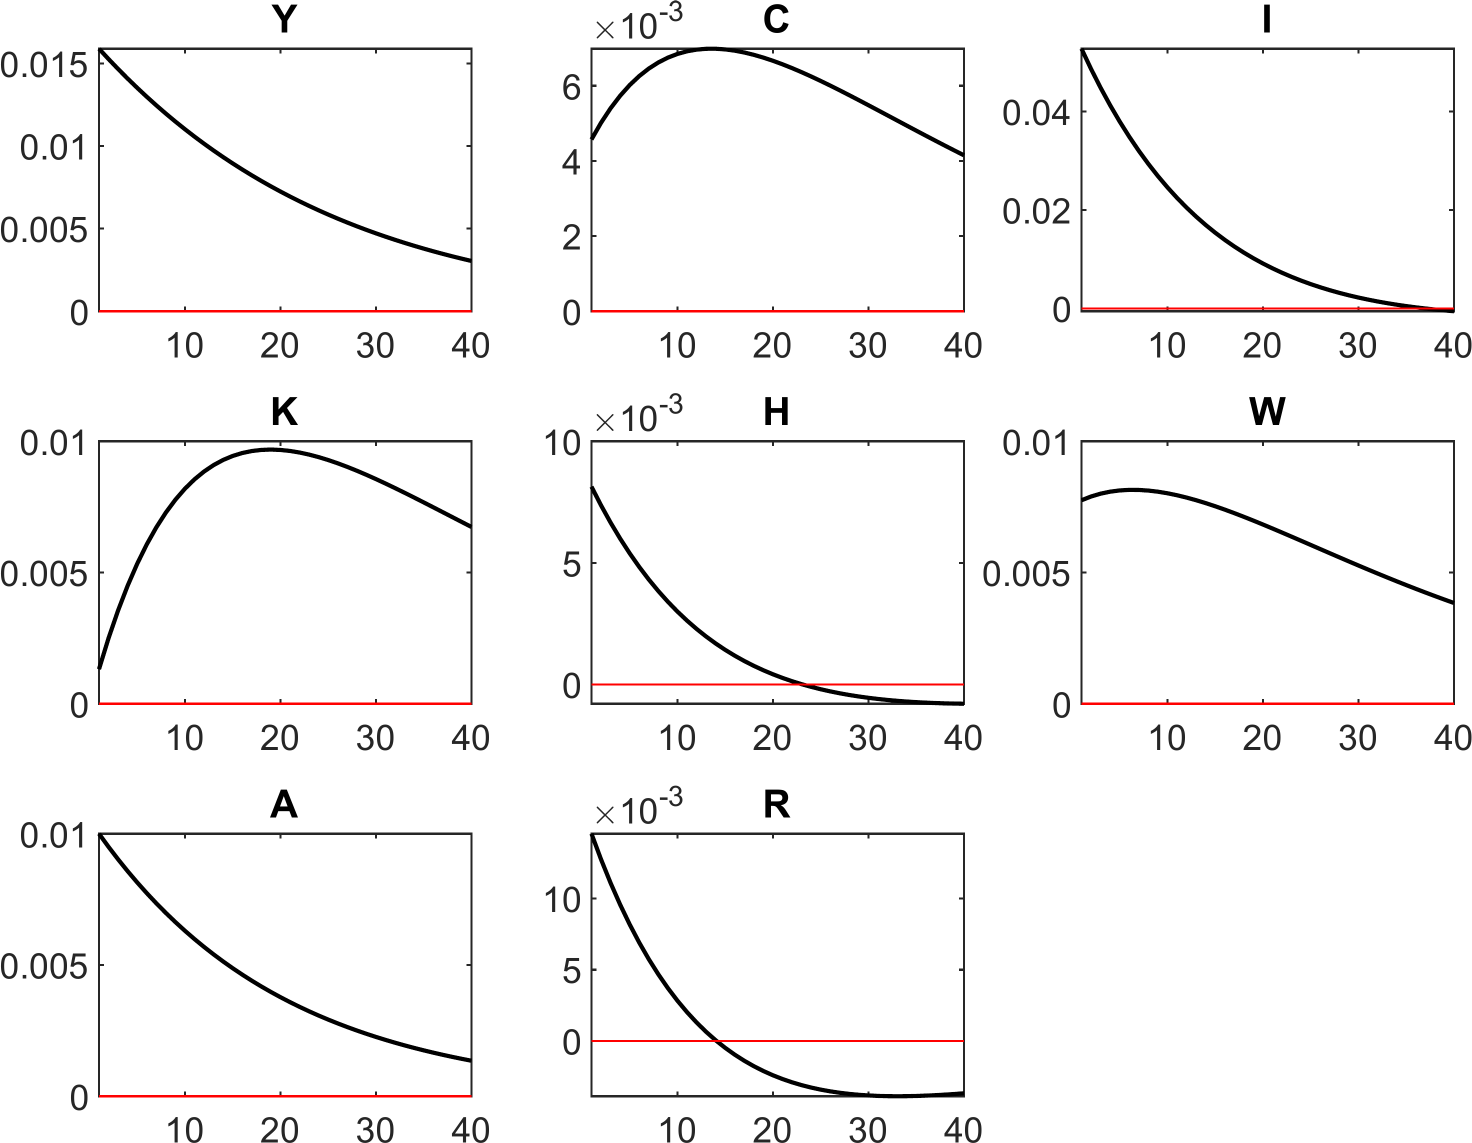
\includegraphics{code/rbc_model/rbc_model/graphs/rbc_model_IRF_eps_cropped.png}
\caption{image}
\end{figure}

\newpage

\section{Appendix}\label{appendix}

\subsection{Households}\label{households-1}

\begin{align*}
  & \text{Define Lagrangian} \\
  & \mathcal{L} = \mathbb{E}_0 \sum_{t=1}^{\infty} \beta^{t-1} \Bigl\{
    \underbrace{\frac{\bigl(c_t-\eta \, c_{t-1}\bigr)^{1-\theta}}{1-\theta}}_{\text{Consumption utility}}
    - \underbrace{\chi\frac{h_t^{1+\gamma}}{1+\gamma}}_{\text{Labour disutility}}
    + \underbrace{\psi\ln\bigl(m_t\bigr)}_{\text{Money utility}} \\
  & \quad\qquad
    + \underbrace{\lambda_t\bigl[\dfrac{R^B_{t-1}b_{t-1}}{\pi_t} + \dfrac{m_{t-1}}{\pi_t} + w_t h_t + r^k_t K_{t-1} + \Pi^r_t - \tau_t -c_t - i_t - b_t - m_t\bigr]}_{\text{Real flow constraint}}
    + \underbrace{\mu_t\bigl[(1 - \delta)\,K_{t-1}
\;+\; i_t
\;-\;\frac{\phi_k}{2}
\left(\frac{i_t}{K_{t-1}} - \delta\right)^{2}
\,K_{t-1} - K_t]}_{\text{Capital accumulation}}
  \Bigr\}
\end{align*}

\subsubsection{\texorpdfstring{First Order Conditions
\label{household_FOC}}{First Order Conditions }}\label{first-order-conditions}

FOC w.r.t. Consumption

\begin{align*}
  & \frac{\partial \mathcal{L}}{\partial c_t} = 0 \\
  & \quad \bigl[(c_t-\eta c_{t-1})^{-\theta} - \lambda_t\bigr] 
    - \beta\,\eta\,\mathbb{E}_t\bigl[(c_{t+1}-\eta c_t)^{-\theta}\bigr] = 0 \\[6pt]
  & \text{Rearrange} \\
  & \quad \lambda_t = (c_t-\eta c_{t-1})^{-\theta} - \beta\,\eta\,\mathbb{E}_t\bigl[(c_{t+1}-\eta c_t)^{-\theta}\bigr]
\end{align*}

\begin{equation}\label{foc_C_app}
\boxed{\lambda_t = (c_t-\eta c_{t-1})^{-\theta} - \beta\,\eta\,\mathbb{E}_t\bigl[(c_{t+1}-\eta c_t)^{-\theta}\bigr]}
\end{equation}

FOC w.r.t. Labour \begin{align*}
  & \frac{\partial \mathcal{L}}{\partial h_t} = 0 \\
  & \quad -\chi h_t^{\gamma} + \lambda_t w_t = 0 \\[6pt]
  & \text{Rearrange} \\
  & \quad \lambda_t w_t = \chi h_t^{\gamma}
\end{align*}

\begin{equation}\label{foc_h_app}
\boxed{\lambda_t w_t = \chi h_t^{\gamma}}
\end{equation}

FOC w.r.t. Real Bonds: \begin{align*}
  & \frac{\partial \mathcal{L}}{\partial b_t} = 0 \\
  & \quad -\beta^{t-1} \lambda_t + \beta^{t} \, \mathbb{E}_t \left[ \lambda_{t+1} \cdot \dfrac{R^B_t}{\pi_{t+1}} \right] = 0 \\[6pt]
  & \text{Divide by } \beta^{t-1} \\
  & \quad -\lambda_t + \beta \, \mathbb{E}_t \left[ \lambda_{t+1} \dfrac{R^B_t}{\pi_{t+1}} \right] = 0
\end{align*}

\begin{equation}\label{foc_B_app}
\boxed{\lambda_t = \beta \, \mathbb{E}_t \left[ \lambda_{t+1} \dfrac{R^B_t}{\pi_{t+1}} \right]}
\end{equation}

FOC w.r.t. Real Money Balances: \begin{align*}
  & \frac{\partial \mathcal{L}}{\partial m_t} = 0 \\
  & \quad \beta^{t-1} \left[ \dfrac{\psi}{m_t} - \lambda_t \right] + \beta^{t} \, \mathbb{E}_t \left[ \lambda_{t+1} \cdot \dfrac{1}{\pi_{t+1}} \right] = 0 \\[6pt]
  & \text{Divide by } \beta^{t-1} \\
  & \quad \dfrac{\psi}{m_t} - \lambda_t + \beta \, \mathbb{E}_t \left[ \dfrac{\lambda_{t+1}}{\pi_{t+1}} \right] = 0
\end{align*}

\begin{equation}\label{foc_M_app}
\boxed{\dfrac{\psi}{m_t} = \lambda_t - \beta \, \mathbb{E}_t \left[ \dfrac{\lambda_{t+1}}{\pi_{t+1}} \right]}
\end{equation}

FOC w.r.t. Investment: \begin{align*}
  & \frac{\partial \mathcal{L}}{\partial i_t} = 0 \\
  & \quad \beta^{t-1} \left[ -\lambda_t + \mu_t \cdot \frac{\partial}{\partial i_t} \left( i_t - \frac{\phi_k}{2} \left( \frac{i_t}{K_{t-1}} - \delta \right)^2 K_{t-1} \right) \right] = 0 \\[6pt]
  & \text{Compute derivative:} \\
  & \quad \frac{\partial}{\partial i_t} \left[ i_t - \frac{\phi_k}{2} \left( \frac{i_t}{K_{t-1}} - \delta \right)^2 K_{t-1} \right] = 1 - \phi_k \left( \frac{i_t}{K_{t-1}} - \delta \right) \\[6pt]
  & \text{Substitute and simplify:} \\
  & \quad -\lambda_t + \mu_t \left( 1 - \phi_k \left( \frac{i_t}{K_{t-1}} - \delta \right) \right) = 0
\end{align*}

\begin{equation}\label{foc_I_app}
\boxed{\lambda_t = \mu_t \left( 1 - \phi_k \left( \frac{i_t}{K_{t-1}} - \delta \right) \right)}
\end{equation}

FOC w.r.t. Capital: \begin{align*}
  & \frac{\partial \mathcal{L}}{\partial K_t} = 0 \\
  & \quad \beta^{t-1} (-\mu_t) + \beta^{t} \, \mathbb{E}_t \left[ \lambda_{t+1} r^k_{t+1} + \mu_{t+1} \cdot \frac{\partial}{\partial K_t} \left( (1-\delta) K_t + i_{t+1} - \frac{\phi_k}{2} \left( \frac{i_{t+1}}{K_t} - \delta \right)^2 K_t \right) \right] = 0 \\[6pt]
  & \text{Compute derivative:} \\
  & \quad \frac{\partial}{\partial K_t} \left[ (1-\delta) K_t - \frac{\phi_k}{2} \left( \frac{i_{t+1}}{K_t} - \delta \right)^2 K_t \right] = (1-\delta) - \frac{\phi_k}{2} \left( \delta^2 - \left( \frac{i_{t+1}}{K_t} \right)^2 \right) \\[6pt]
  & \text{Substitute and simplify:} \\
  & \quad -\mu_t + \beta \, \mathbb{E}_t \left[ \lambda_{t+1} r^k_{t+1} + \mu_{t+1} \left( (1-\delta) - \frac{\phi_k}{2} \left( \delta^2 - \left( \frac{i_{t+1}}{K_t} \right)^2 \right) \right) \right] = 0
\end{align*}

\begin{equation}\label{foc_K_app}
\boxed{\mu_t = \beta \, \mathbb{E}_t \left[ \lambda_{t+1} r^k_{t+1} + \mu_{t+1} \left( (1-\delta) - \frac{\phi_k}{2} \left( \delta^2 - \left( \frac{i_{t+1}}{K_t} \right)^2 \right) \right) \right]}
\end{equation}

\newpage

\subsection{Production}\label{production-1}

\subsubsection{\texorpdfstring{Final Good Producer
\label{final_good_producer_appendix}}{Final Good Producer }}\label{final-good-producer}

\textbf{Derivation of Intermediate Goods Demand and Aggregate Price
Index}

\begin{align*}  
& \text{Final goods producer's profit:} \\  
& \Pi_t = P_t Y_t - \int_0^1 P_t(j) Y_t(j)  dj \\  
& \text{subject to } Y_t = \left( \int_0^1 Y_t(j)^{\frac{\epsilon-1}{\epsilon}}  dj \right)^{\frac{\epsilon}{\epsilon-1}} \\  
& \\  
& \text{Substitute production function into profit:} \\  
& \Pi_t = P_t \left( \int_0^1 Y_t(j)^{\frac{\epsilon-1}{\epsilon}}  dj \right)^{\frac{\epsilon}{\epsilon-1}} - \int_0^1 P_t(j) Y_t(j)  dj \\  
& \\  
& \text{First-order condition for } Y_t(j): \\  
& \frac{\partial \Pi_t}{\partial Y_t(j)} = P_t \cdot \frac{\epsilon}{\epsilon-1} \left( \int_0^1 Y_t(i)^{\frac{\epsilon-1}{\epsilon}}  di \right)^{\frac{1}{\epsilon-1}} \cdot \frac{\epsilon-1}{\epsilon} Y_t(j)^{-\frac{1}{\epsilon}} - P_t(j) = 0 \\  
& \Rightarrow P_t \cdot Y_t^{\frac{1}{\epsilon}} Y_t(j)^{-\frac{1}{\epsilon}} = P_t(j) \\  
& \\  
& \text{Rearrange to obtain demand curve:} \\  
& Y_t(j) = \left( \frac{P_t}{P_t(j)} \right)^{\epsilon} Y_t \\  
& \\  
& \text{Substitute demand into production function:} \\  
& Y_t = \left( \int_0^1 \left[ \left( \frac{P_t}{P_t(j)} \right)^{\epsilon} Y_t \right]^{\frac{\epsilon-1}{\epsilon}}  dj \right)^{\frac{\epsilon}{\epsilon-1}} \\  
& = Y_t \left( \int_0^1 \left( \frac{P_t}{P_t(j)} \right)^{\epsilon-1}  dj \right)^{\frac{\epsilon}{\epsilon-1}} \\  
& \\
\end{align*}

\begin{align*} 
& \text{Simplify to obtain price index:} \\  
& 1 = \left( \int_0^1 \left( \frac{P_t}{P_t(j)} \right)^{\epsilon-1}  dj \right)^{\frac{\epsilon}{\epsilon-1}} \\  
& \Rightarrow P_t^{1-\epsilon} = \int_0^1 P_t(j)^{1-\epsilon}  dj \\  
& \Rightarrow P_t = \left( \int_0^1 P_t(j)^{1-\epsilon}  dj \right)^{\frac{1}{1-\epsilon}}  
\end{align*}

\begin{equation}\label{demand_and_price}  
\boxed{  
  \begin{gathered}  
  Y_t(j) = \left( \frac{P_t(j)}{P_t} \right)^{-\epsilon} Y_t \\  
  \\  
  P_t = \left( \int_0^1 P_t(j)^{1-\epsilon}  dj \right)^{\frac{1}{1-\epsilon}}  
  \end{gathered}  
}  
\end{equation}

\subsubsection{\texorpdfstring{Intermediate Goods Producers
\label{intermediate_good_producer_appendix}}{Intermediate Goods Producers }}\label{intermediate-goods-producers-1}

\begin{align*}
& \text{Cost minimization for intermediate firm } j: \\
& \min_{K_t(j), h_t(j)} \left\{ r_t^k K_t(j) + w_t h_t(j) \right\} \\
& \text{subject to } Y_t(j) = A_t K_t(j)^{\alpha} h_t(j)^{1-\alpha} \\
& \\
& \text{Lagrangian:} \\
& \mathcal{L} = r_t^k K_t(j) + w_t h_t(j) + \lambda_t \left[ A_t K_t(j)^{\alpha} h_t(j)^{1-\alpha} - Y_t(j) \right] \\
& \\
& \text{First-order conditions:} \\
& \frac{\partial \mathcal{L}}{\partial K_t(j)} = 0: \quad r_t^k = \lambda_t \alpha A_t K_t(j)^{\alpha-1} h_t(j)^{1-\alpha} \\
& \frac{\partial \mathcal{L}}{\partial h_t(j)} = 0: \quad w_t = \lambda_t (1-\alpha) A_t K_t(j)^{\alpha} h_t(j)^{-\alpha} \\
& \\
& \text{Rearrange FOCs:} \\
& \lambda_t = \frac{r_t^k}{\alpha} \left( \frac{K_t(j)}{h_t(j)} \right)^{1-\alpha} \frac{1}{A_t}, \quad 
\lambda_t = \frac{w_t}{1-\alpha} \left( \frac{K_t(j)}{h_t(j)} \right)^{\alpha} \frac{1}{A_t} \\
& \\
& \text{Equate expressions:} \\
& \frac{r_t^k}{\alpha} \left( \frac{K_t(j)}{h_t(j)} \right)^{-\alpha} = \frac{w_t}{1-\alpha} \left( \frac{K_t(j)}{h_t(j)} \right)^{1-\alpha} \\
& \Rightarrow \frac{K_t(j)}{h_t(j)} = \frac{\alpha}{1-\alpha} \frac{w_t}{r_t^k} \\
& \\
& \text{Substitute into capital FOC:} \\
& \lambda_t = \frac{r_t^k}{\alpha A_t} \left( \frac{\alpha}{1-\alpha} \frac{w_t}{r_t^k} \right)^{\alpha-1} \\
& = \frac{1}{A_t} \left( \frac{r_t^k}{\alpha} \right)^{\alpha} \left( \frac{w_t}{1-\alpha} \right)^{1-\alpha}
\end{align*}

\begin{equation}\label{marginal_cost_appendix}
\boxed{mc_t = \dfrac{1}{A_t} \left( \dfrac{r_t^k}{\alpha} \right)^{\alpha} \left( \dfrac{w_t}{1-\alpha} \right)^{1-\alpha}}
\end{equation}

\begin{align*}
& \text{Intermediate‐goods producer’s problem:} \\
& \max_{P_t(j)} \;\mathbb{E}_t \sum_{s=0}^{\infty} \Lambda_{t,t+s}
  \Bigl[
    \bigl(\tfrac{P_{t+s}(j)}{P_{t+s}}\bigr)^{1-\epsilon} Y_{t+s}
    - mc_{t+s}\,\bigl(\tfrac{P_{t+s}(j)}{P_{t+s}}\bigr)^{-\epsilon} Y_{t+s}
    - \tfrac{\phi_p}{2}\bigl(\tfrac{P_{t+s}(j)}{P_{t+s-1}(j)} - 1\bigr)^2 Y_{t+s}
  \Bigr] \\
& \text{subject to} \quad Y_t(j) = \bigl(\tfrac{P_t(j)}{P_t}\bigr)^{-\epsilon} Y_t
\\[1.5ex]
& \text{First‐Order Condition w.r.t. }P_t(j): \\
& \mathbb{E}_t\Bigl[
    \frac{\partial \Pi_t(j)}{\partial P_t(j)}
    + \beta\,\Lambda_{t,t+1}
      \frac{\partial \Pi_{t+1}(j)}{\partial P_t(j)}
  \Bigr] = 0
\\[1ex]
& \frac{\partial \Pi_t}{\partial P_t(j)}
  = (1-\epsilon)\bigl(\tfrac{P_t(j)}{P_t}\bigr)^{-\epsilon}\tfrac{Y_t}{P_t}
    + \epsilon\,mc_t\bigl(\tfrac{P_t(j)}{P_t}\bigr)^{-\epsilon-1}\tfrac{Y_t}{P_t}
    - \phi_p\bigl(\tfrac{P_t(j)}{P_{t-1}(j)}-1\bigr)\tfrac{Y_t}{P_{t-1}(j)}
\\[1ex]
& \frac{\partial \Pi_{t+1}}{\partial P_t(j)}
  = \phi_p\bigl(\tfrac{P_{t+1}(j)}{P_t(j)}-1\bigr)\,\tfrac{P_{t+1}(j)}{P_t(j)^2}\,Y_{t+1}
\\[2ex]
& \text{Impose symmetry: }P_t(j)=P_t,\;Y_t(j)=Y_t,\;\pi_t=\tfrac{P_t}{P_{t-1}}.\\
& (1-\epsilon)+\epsilon\,mc_t = \epsilon\bigl(mc_t-\tfrac{\epsilon-1}{\epsilon}\bigr),\quad
  \tfrac{P_t(j)}{P_{t-1}(j)}=\pi_t,\;\tfrac{P_{t+1}(j)}{P_t(j)}=\pi_{t+1}
\\[1ex]
& 0 = \epsilon\bigl(mc_t-\tfrac{\epsilon-1}{\epsilon}\bigr)
      - \phi_p\,(\pi_t-1)\,\pi_t
      + \beta\,\mathbb{E}_t\Bigl[
          \Lambda_{t,t+1}\,\phi_p\,(\pi_{t+1}-1)\,\pi_{t+1}
          \,\tfrac{Y_{t+1}P_t}{Y_tP_{t+1}}
        \Bigr]
\\[1ex]
\end{align*}

Noting \(\Lambda_{t,t+1}=\beta\,\tfrac{\lambda_{t+1}}{\lambda_t}\) and
\(P_{t+1}/P_t=\pi_{t+1}\), the bracket simplifies to
\(\beta\,\tfrac{\lambda_{t+1}}{\lambda_t}\,\tfrac{Y_{t+1}}{Y_t}\).

\begin{equation}\label{rotemberg_FOC}
\boxed{
  0 = \epsilon\Bigl(mc_t - \tfrac{\epsilon-1}{\epsilon}\Bigr)
      - \phi_p\,(\pi_t - 1)\,\pi_t
      + \beta\,\mathbb{E}_t\!
        \Bigl[
          \tfrac{\lambda_{t+1}}{\lambda_t}\,
          \phi_p\,(\pi_{t+1}-1)\,\pi_{t+1}\,
          \tfrac{Y_{t+1}}{Y_t}
        \Bigr]
}
\end{equation}

\subsection{\texorpdfstring{Steady State
\label{steady_state_app}}{Steady State }}\label{steady-state-1}

\begin{align*}
\max_{P_t(j)}\;&(P_t(j)/P_t)^{1-\epsilon}Y_t \;-\; mc_t\,(P_t(j)/P_t)^{-\epsilon}Y_t \\[6pt]
\frac{\partial}{\partial P_t(j)}:\;&(1-\epsilon)(P_t(j)/P_t)^{-\epsilon}\frac{Y_t}{P_t}
\;+\;\epsilon\,mc_t\,(P_t(j)/P_t)^{-\epsilon-1}\frac{Y_t}{P_t}=0 \\[6pt]
\Rightarrow\;&(1-\epsilon)+\epsilon\,mc_t\,(P_t(j)/P_t)^{-1}=0 \\[4pt]
\Rightarrow\;&P_t(j)/P_t=\frac{\epsilon}{\epsilon-1}\;mc_t
\end{align*}

In equilibrium \(P_t(j)=P_t\), so \[
1=\frac{\epsilon}{\epsilon-1}\,mc_t
\] \begin{equation}\label{eq:mc}
mc^*_t=\frac{\epsilon-1}{\epsilon}
\end{equation}

\subsubsection{Derivation of Flexible-Price Steady-State
Values}\label{derivation-of-flexible-price-steady-state-values}

\begin{align*}
& \text{Factor Prices and Technology Link} \\
& mc^* = \frac{\epsilon - 1}{\epsilon} \\
& mc^* = \frac{1}{A} \left( \frac{r^{k,*}}{\alpha} \right)^{\alpha}
            \left( \frac{w^*}{1-\alpha} \right)^{1-\alpha} \\
& \text{Substitute to get} \\
& \frac{\epsilon - 1}{\epsilon}
  = \frac{1}{A} \left( \frac{r^{k,*}}{\alpha} \right)^{\alpha}
    \left( \frac{w^*}{1-\alpha} \right)^{1-\alpha}
\end{align*}

\begin{align*}
& \text{Steady-State Real Rates} \\
& r^{B,*} = \frac{1}{\beta} \\
& r^{k,*} = \frac{1}{\beta} - (1 - \delta)
\end{align*}

\begin{align*}
& \text{Solve for Wage } w^* \\
& \frac{K^*}{h^*}
  = \Bigl(\tfrac{mc^*\,\alpha\,A}{r^{k,*}}\Bigr)^{\!\frac{1}{1-\alpha}} \\
& w^* = mc^*(1-\alpha)\,A \Bigl(\tfrac{K^*}{h^*}\Bigr)^{\!\alpha} \\
& \text{Substitute to get} \\
& w^* = \frac{\epsilon-1}{\epsilon}\,(1-\alpha)\,A
         \Bigl(\tfrac{\tfrac{\epsilon-1}{\epsilon}\,\alpha\,A}
                     {\tfrac{1}{\beta} - (1-\delta)}\Bigr)^{\!\frac{\alpha}{1-\alpha}}
\end{align*}

\begin{align*}
& \text{labour Supply with Habit Formation} \\
& \lambda^* = [c^*(1-\eta)]^{-\theta}(1 - \beta\eta) \\
& [c^*(1-\eta)]^{-\theta}(1 - \beta\eta)\,w^* = \chi\,(h^*)^\gamma
\end{align*}

\begin{align*}
& \text{Resource Constraints} \\
& i^* = \delta K^* \\
& Y^* = c^* + i^* + \bar{g} = c^* + \delta K^* + \bar{g}
\end{align*}

\begin{align*}
& \text{Solve for Steady-State Values} \\
& Y^* = A (K^*)^\alpha (h^*)^{1-\alpha} \\
& k \equiv \tfrac{K^*}{h^*}
  = \Bigl(\tfrac{\tfrac{\epsilon-1}{\epsilon}\,\alpha\,A}
               {\tfrac{1}{\beta} - (1-\delta)}\Bigr)^{\!\frac{1}{1-\alpha}} \\
& Y^* = A k^\alpha h^* \\
& A k^\alpha h^* = \frac{1}{1-\eta}
                   \Bigl(\tfrac{(1-\beta\eta)\,w^*}{\chi}\Bigr)^{\!\frac{1}{\theta}}
                   (h^*)^{-\frac{\gamma}{\theta}}
                 + \delta k h^* + \bar{g}
\end{align*}

\begin{align*}
& \Omega \equiv \frac{1}{1-\eta}
                 \Bigl(\tfrac{(1-\beta\eta)\,w^*}{\chi}\Bigr)^{\!\frac{1}{\theta}}, 
\quad
D \equiv A k^\alpha - \delta k \\
& D\,h^* - \bar{g} = \Omega\,(h^*)^{-\frac{\gamma}{\theta}}
\end{align*}

\begin{align*}
& \text{ Monetary Policy Steady State} \\
& \pi^* = \pi_* \\
& R^* = r^{B,*}\,\pi^* = \frac{\pi_*}{\beta}
\end{align*}

\begin{equation}\label{closed_form_ss}
\boxed{
  \begin{gathered}
    k = \Bigl(\tfrac{\tfrac{\epsilon-1}{\epsilon}\,\alpha\,A}
                  {\tfrac{1}{\beta} - (1-\delta)}\Bigr)^{\!\frac{1}{1-\alpha}},
    \quad
    w^* = \tfrac{\epsilon-1}{\epsilon}(1-\alpha)\,A\,k^\alpha, \\[6pt]
    h^*:\; D\,h^* - \bar{g} = \Omega\,(h^*)^{-\gamma/\theta}, 
    \quad
    K^* = k\,h^*, 
    \\[4pt]
    Y^* = A\,k^\alpha\,h^*, 
    \quad 
    c^* = D\,h^* - \bar{g}, 
    \quad 
    i^* = \delta\,k\,h^*,
    \\[4pt]
    \Omega = \tfrac{1}{1-\eta}
             \Bigl(\tfrac{(1-\beta\eta)\,w^*}{\chi}\Bigr)^{\!\tfrac{1}{\theta}},
    \quad
    D = A\,k^\alpha - \delta\,k
  \end{gathered}
}
\end{equation}

\newpage

\section*{References}\label{references}
\addcontentsline{toc}{section}{References}

\phantomsection\label{refs}
\begin{CSLReferences}{1}{1}
\bibitem[\citeproctext]{ref-ecbwp770}
European Central Bank. 2022. \emph{Economic and monetary developments
no. 770}. (ECB Working Paper 770). European Central Bank. {[}Online{]},
Available: \url{https://www.ecb.europa.eu/pub/pdf/scpwps/ecbwp770.pdf}.

\bibitem[\citeproctext]{ref-Mati2019}
Mati, S. 2019. DynareR: Bringing the power of {Dynare} to {R}, {R
Markdown}, and {Quarto}. \emph{CRAN}. {[}Online{]}, Available:
\url{https://CRAN.R-project.org/package=DynareR}.

\bibitem[\citeproctext]{ref-sims2024newkeynesian}
Sims, E. 2024a. \emph{Graduate macro theory II: The basic new keynesian
model}. (Lecture Notes ECON 60202 -- Spring 2024). Notre Dame, IN:
University of Notre Dame. {[}Online{]}, Available:
\url{https://sites.nd.edu/esims/files/2024/03/notes_new_keynesian_2024-1.pdf}.

\bibitem[\citeproctext]{ref-sims2024rbc}
Sims, E. 2024b. \emph{Graduate macro theory II: Extensions of basic RBC
framework}. (Lecture Notes ECON 60202 -- Spring 2024). Notre Dame, IN:
University of Notre Dame. {[}Online{]}, Available:
\url{https://sites.nd.edu/esims/files/2024/02/notes_rbc_extensions_2024.pdf}.

\bibitem[\citeproctext]{ref-sims2024fiscal}
Sims, E. 2024c. \emph{Fiscal policy in the RBC model}. (Lecture Notes
ECON 60202 -- Spring 2024). Notre Dame, IN: University of Notre Dame.
{[}Online{]}, Available:
\url{https://sites.nd.edu/esims/files/2024/02/notes_fiscal_policy_2024.pdf}.

\end{CSLReferences}

\bibliography{Tex/ref}





\end{document}
